\section{Methodology}
\label{sec:methodology}

This section describes our analytical framework, organized into four components: road network association (Section~\ref{sec:meth_road}), safety-relevant speed indicator computation (Section~\ref{sec:meth_indicators}), spatial analysis of speed behavior (Section~\ref{sec:meth_spatial}), and statistical modeling (Section~\ref{sec:meth_models}).

\subsection{Road Network Association}
\label{sec:meth_road}

To link e-scooter speed behavior with road infrastructure attributes, we associate each GPS trajectory with the underlying road network. We extracted the OpenStreetMap (OSM) road network for all 50 cities with at least 5,000 trips using \texttt{osmnx} v2.0 \citep{boeing2017osmnx}. The combined network comprises 1.32~million nodes and 3.57~million edges. Each edge carries an OSM \texttt{highway} tag indicating the road functional class, which we mapped to 11 categories: motorway, trunk, primary, secondary, tertiary, unclassified, residential, service, footway, cycleway, and path.

For road class assignment, we evaluated two approaches. First, we tested Hidden Markov Model (HMM)-based map-matching using the Leuven Map Matching library \citep{meert2018hmm}, which achieves 100\% match rates on a validation sample of 200 Seoul trips but requires approximately 5.8~seconds per trip---rendering full-dataset processing infeasible for 2.78~million trajectories. Second, we implemented a nearest-edge approach using a spatial KD-tree index constructed from the OSM edge midpoints. For each GPS point in a trip, we identify the nearest road edge and extract its \texttt{highway} tag. This approach processes the full dataset (105~million GPS points across 2,775,170 trips) in 463~seconds. While nearest-edge assignment lacks the topological consistency of HMM-based matching---particularly at complex intersections with parallel roads---we validated the results by confirming that per-trip road class fractions sum to 1.0, that spatial patterns are geographically consistent (e.g., higher major-road fractions in central urban areas), and that the dominant road class distribution aligns with known Korean urban morphology (Figure~\ref{fig:map_matching}, Appendix).

From the road class assignment, we derive several per-trip infrastructure features:
\begin{itemize}
    \item $\text{frac}_{c}$: fraction of GPS points on road class $c$ (11 features);
    \item $\text{frac\_major\_road}$: fraction on motorway, trunk, primary, or secondary roads;
    \item $\text{frac\_cycling\_infra}$: fraction on cycleway or path segments;
    \item $\text{dominant\_road\_class}$: the road class with the highest point fraction;
    \item $\text{n\_road\_classes}$: count of distinct road classes traversed.
\end{itemize}

We note that OSM speed limit (\texttt{maxspeed}) coverage in South Korea is very low (1--12\% of edges depending on city), precluding road-specific speed limit analysis. The \texttt{highway} functional class, which has 100\% coverage, serves as the primary road infrastructure variable throughout our analysis.

\subsection{Safety-Relevant Speed Indicators}
\label{sec:meth_indicators}

We define and compute a multi-level suite of speed-based safety indicators, summarized in Table~\ref{tab:indicators}. All indicators are derived from the onboard speed sensor data (the \texttt{speeds} column), which records speed at approximately 10-second intervals.

\subsubsection{Trip-Level Indicators}

For each trip $i$ with speed vector $\mathbf{v}_i = (v_{i1}, \ldots, v_{iT_i})$, we compute mean speed, maximum speed, P85 speed, speed coefficient of variation ($\text{CV}_i = \sigma_i / \bar{v}_i$), speeding rate ($r_i = T_i^{-1} \sum_t \mathbf{1}(v_{it} > 25)$), and binary speeding indicator ($\text{is\_speeding}_i = \mathbf{1}(v_i^{\max} > 25)$). We also compute $r_i$ at alternative thresholds of 20 and 30~km/h for sensitivity analysis.

\subsubsection{Acceleration and Within-Trip Features}

Longitudinal acceleration is computed as $a_{it} = (v_{i,t+1} - v_{it}) / \Delta t$ with $\Delta t \approx 10$~s. We define harsh events at $|a| > 0.5$~m/s$^2$, calibrated for our coarse temporal resolution (the 2.0~m/s$^2$ automotive threshold is unreachable at 10-second intervals). Within-trip profile features include cruise fraction (proportion within $\pm 3$~km/h of median speed), zero-speed fraction, and first-half vs.\ second-half speed ratio. Figure~\ref{fig:speed_profile} illustrates the extraction process for a sample trip.

\subsubsection{User-Level Indicators}

For each user $u$, we aggregate trip-level indicators to compute user mean speed, speeding propensity (fraction of trips with any speeding), speed consistency (variance of trip mean speeds), and harsh event propensity.

% Indicator summary table
\begin{table}[htbp]
\centering
\caption{Safety-relevant speed indicators: definitions and levels of analysis.}
\label{tab:indicators}
\small
\begin{tabular}{llll}
\toprule
\textbf{Indicator} & \textbf{Level} & \textbf{Formula} & \textbf{Unit} \\
\midrule
Mean speed & Trip & $\bar{v}_i = \frac{1}{T_i} \sum_t v_{it}$ & km/h \\
Maximum speed & Trip & $v_i^{\max} = \max_t v_{it}$ & km/h \\
P85 speed & Trip & 85th percentile of $\mathbf{v}_i$ & km/h \\
Speed CV & Trip & $\sigma_i / \bar{v}_i$ & --- \\
Speeding rate & Trip & $\frac{1}{T_i} \sum_t \mathbf{1}(v_{it} > 25)$ & --- \\
Harsh accel.\ count & Trip & $\sum_t \mathbf{1}(a_{it} > 0.5)$ & events \\
Cruise fraction & Trip & frac.\ within $\pm$3 km/h of median & --- \\
Zero-speed fraction & Trip & $\frac{1}{T_i} \sum_t \mathbf{1}(v_{it} = 0)$ & --- \\
\addlinespace
User mean speed & User & $\frac{1}{|\mathcal{T}_u|} \sum_i \bar{v}_i$ & km/h \\
Speeding propensity & User & frac.\ of trips with max $> 25$ & --- \\
Harsh event propensity & User & frac.\ of trips with harsh events & --- \\
Speed consistency & User & var.\ of trip mean speeds & (km/h)$^2$ \\
\addlinespace
Hex speeding rate & Spatial & mean of trip-level speeding rates in hex & --- \\
Hex trip density & Spatial & trip count per H3 hex cell & trips \\
\bottomrule
\end{tabular}
\end{table}

\begin{figure}[htbp]
\centering
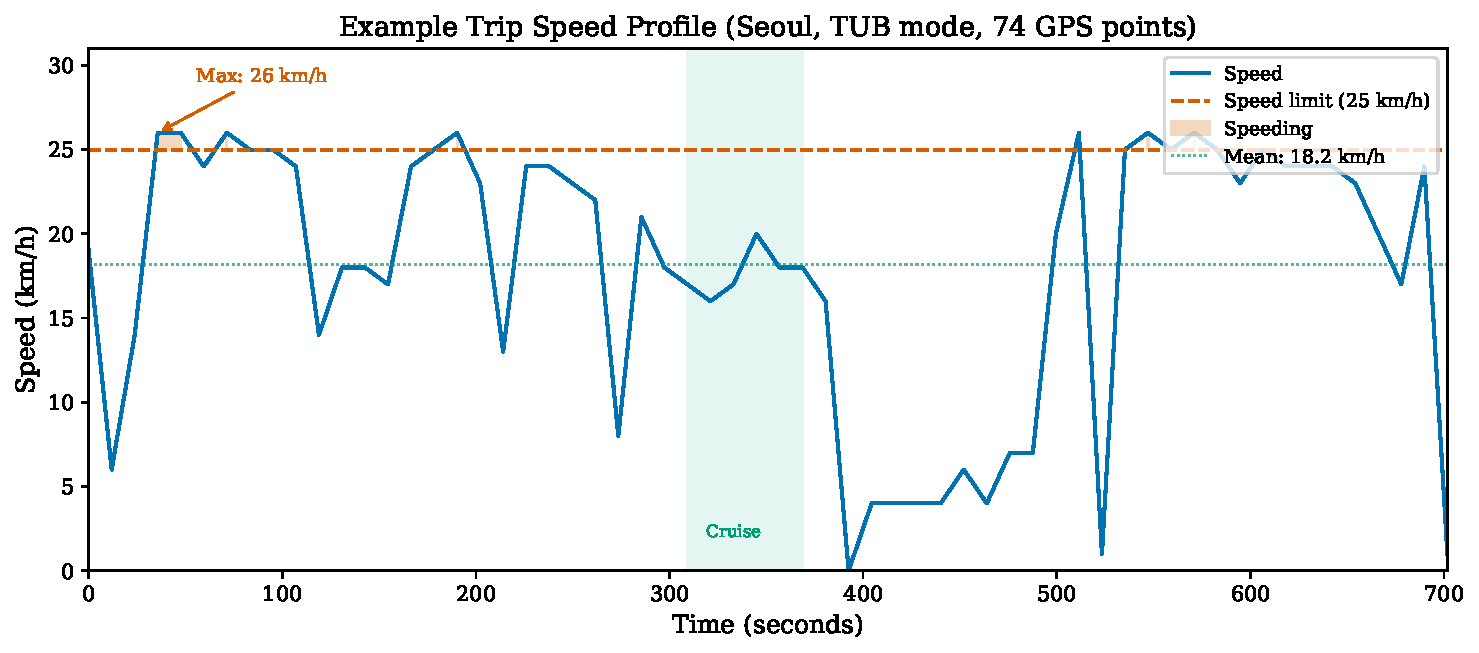
\includegraphics[width=\textwidth]{figures/fig3_speed_profile_example.pdf}
\caption{Illustration of within-trip speed profile extraction and safety indicator computation for a sample TUB-mode trip in Seoul. The horizontal dashed line indicates the 25~km/h regulatory speed limit; shaded regions indicate speeding episodes. Annotated indicators include mean speed, cruise region, and harsh acceleration/deceleration events.}
\label{fig:speed_profile}
\end{figure}

\subsection{Spatial Analysis of Speed Behavior}
\label{sec:meth_spatial}

\subsubsection{Hexagonal Grid Aggregation}

We aggregate trip-level indicators to the H3 hexagonal grid \citep{h3uber} at resolution 8 ($\sim$461~m edge, $\sim$0.74~km$^2$), assigning trips by origin coordinates. Hexagonal tessellation provides uniform adjacency, producing more stable spatial statistics than rectangular grids \citep{birch2007rectangular}. After filtering to cells with $\geq$10 trips, 6,111 of 8,144 cells remain. Per-hex indicators include mean speeding rate, trip count, and merged road infrastructure attributes.

\subsubsection{Spatial Autocorrelation and Hotspot Detection}

We assess global spatial autocorrelation using Moran's $I$ \citep{moran1950notes} with $k$-nearest neighbor weights ($k = 8$, 999 permutations). We identify spatial clusters using the Getis-Ord $G_i^*$ statistic \citep{getis1992analysis}, classifying cells as hot spots or cold spots at $p < 0.05$ (FDR-corrected), conducted separately for five cities. We additionally apply LISA \citep{anselin1995local} to classify hexes into HH, LL, HL, and LH clusters.

\subsection{Statistical Modeling}
\label{sec:meth_models}

We estimate four complementary statistical models to address different aspects of speed behavior. Table~\ref{tab:model_specs} summarizes the model specifications.

\subsubsection{Model 1: Logistic Regression with GEE for Speeding Propensity}
\label{sec:meth_m1}

We model binary speeding ($\text{is\_speeding}_i = \mathbf{1}(v_i^{\max} > 25)$) via logistic regression:
\begin{equation}
    \text{logit}\big(P(\text{is\_speeding}_i = 1)\big) = \boldsymbol{x}_i^{\top} \boldsymbol{\beta}
    \label{eq:logistic}
\end{equation}
where $\boldsymbol{x}_i$ includes age group (8 categories; ref: $<$20), operating mode (ref: STD), time of day (5 periods; ref: midday), day type, and province (17; ref: Seoul). We estimate on the full dataset (2.78M trips) and validate with a GEE specification on 200,000 trips using exchangeable working correlation \citep{zeger1986longitudinal} to account for within-user dependence.

\subsubsection{Model 2: Mixed-Effects Linear Model for Mean Speed}
\label{sec:meth_m2}

We model trip-level mean speed with random intercepts for users:
\begin{equation}
    \bar{v}_i = \boldsymbol{x}_i^{\top} \boldsymbol{\beta} + u_{\text{user}(i)} + \epsilon_i, \quad u_{\text{user}(i)} \sim \mathcal{N}(0, \sigma_u^2)
    \label{eq:mixed}
\end{equation}
Fixed effects include Model~1 covariates plus road infrastructure features (dominant road class, $\text{frac\_major\_road}$, log-distance). The ICC $= \sigma_u^2 / (\sigma_u^2 + \sigma^2)$ quantifies between-user variance. Estimated on 100,000 stratified trips with OLS validation on the full dataset.

\subsubsection{Model 3: Two-Part Hurdle Model for Speeding Intensity}
\label{sec:meth_m3}

The speeding rate $r_i \in [0, 1]$ exhibits severe zero-inflation (70.4\% zeros), making standard beta regression inappropriate. We adopt a two-part hurdle model: Part~1 (logistic) models whether any speeding occurs; Part~2 (GLM-binomial, conditional on $r_i > 0$) models intensity. Covariates include mode, age, time, road class, $\text{frac\_major\_road}$, $\text{frac\_cycling\_infra}$, and log-distance. This specification separately identifies factors determining speeding \textit{occurrence} versus \textit{intensity}.

\subsubsection{Model 4: Gaussian Mixture Model for Rider Typology}
\label{sec:meth_m4}

We fit GMMs to 10 standardized user-level speed features (mean/max speed, CV, speeding propensity, speeding rate, acceleration metrics, cruise fraction, zero-speed fraction) for $K = 2, \ldots, 8$. Because BIC does not plateau at $N \approx 198{,}000$, we select $K = 4$ based on interpretability and class separation. Following class assignment, multinomial logistic regression predicts membership from mode, age, province, and trip frequency.

\subsubsection{Natural Experiment: Speed Governor Effectiveness}
\label{sec:meth_natural}

Swing's operating modes create a natural experiment: TUB (no limit), STD ($\sim$20~km/h), and ECO ($\sim$15~km/h) use identical hardware, isolating the software governor as the treatment. For $n = 12{,}046$ users who used both TUB and ECO, we compute paired differences in speed metrics, testing significance with paired $t$-tests and Wilcoxon signed-rank tests, with Cohen's $d$ effect sizes.

% Model specification summary table
\begin{table}[htbp]
\centering
\caption{Summary of statistical model specifications.}
\label{tab:model_specs}
\small
\begin{tabular}{p{1.5cm}p{3cm}p{3.5cm}p{4cm}p{2cm}}
\toprule
\textbf{Model} & \textbf{Outcome} & \textbf{Method} & \textbf{Key Covariates} & \textbf{Sample} \\
\midrule
1 & Binary: any speeding & Logistic + GEE & Age, mode, time, day, province & Full (2.78M) + GEE (200K) \\
\addlinespace
2 & Continuous: mean speed & Mixed-effects linear & Age, mode, time, day, province, road class, frac\_major, log(dist) & Subsample (100K) \\
\addlinespace
3 & Bounded: speeding rate & Two-part hurdle (logistic + GLM-binomial) & Mode, age, time, day, road class, frac\_major, cycling infra & Full (2.78M) \\
\addlinespace
4 & Categorical: rider type & GMM ($K=4$) + multinomial logit & 10 speed behavior features; then mode, age, province, frequency & Users (198K) \\
\addlinespace
5 & Paired: mode effect & Within-subject comparison & TUB vs ECO mode (same users) & 12,046 users \\
\addlinespace
6 & Binary: experience effect & GEE logistic & log(trip\_rank), mode, age, time & 50K users (1.19M trips) \\
\addlinespace
7 & Binary: distance effect & Spline logistic & RCS(log\_dist), road fracs, mode, age & Full (2.32M) \\
\addlinespace
8 & Binary: speeding & LightGBM + SHAP & All features (22) & Full (2.31M) \\
\addlinespace
9 & Continuous: city speeding rate & TWFE DiD + event study & Post $\times$ TUB share, city/month FE & Panel (53 cities $\times$ 11 mo.) \\
\bottomrule
\end{tabular}
\end{table}

\subsubsection{Robustness Checks}
\label{sec:meth_robust}

Robustness checks include threshold sensitivity (20/25/30~km/h), subsampling stability (five 200K-trip subsamples, CV of key ORs), and city-specific models (five largest cities).

\subsection{Extension Analyses}
\label{sec:meth_extensions}

Four extension analyses leverage the full 24-month dataset (44.1M trips, 1.82M users).

\subsubsection{Model 6: Rider Experience and Speeding}
\label{sec:meth_experience}

We compute each user's trip rank and classify riders as newcomers ($\leq$30 calendar days) or established. A GEE logistic regression (50,000 users, 1.19M trips) models speeding as a function of $\log(\text{trip\_rank})$ plus mode, age, and temporal covariates, with a quadratic term to test for non-monotonic effects. Mode-specific newcomer analyses decompose the experience effect into within-mode behavior changes versus mode adoption.

\subsubsection{Model 7: Trip Distance, Road Composition, and Curvature}
\label{sec:meth_distance}

A restricted cubic spline logistic regression captures the non-linear distance--speeding relationship. Road class composition fractions enter as separate covariates. A within-trip speed drift metric ($\bar{v}^{(2)} - \bar{v}^{(1)}$) characterizes speed changes over the trip. Trajectory curvature is computed from GPS bearing changes on 200,000 trips; trips are classified as straight, curvy, or mixed based on sharp-turn fraction ($|\Delta\theta| > 30^\circ$). A composite risk score ($\text{speed\_excess} \times \text{curvature}$) quantifies the risk of speeding on curvy roads.

\subsubsection{Model 8: SHAP Interpretability}
\label{sec:meth_shap}

A LightGBM classifier (80/20 train-test split, 5-fold CV) provides model-agnostic feature importance via SHAP values \citep{lundberg2017unified}. The feature set includes all parametric model covariates plus speed profile features and road class fractions (22 features total).

\subsubsection{Model 9: Difference-in-Differences Causal Analysis}
\label{sec:meth_did}

In December 2023, Swing banned TUB mode system-wide (share: 54.6\% $\rightarrow$ 1.4\%). Because cities varied in pre-ban TUB adoption (32--70\%), we exploit this intensity variation in a DiD design. The panel comprises 53 cities $\times$ 11 months (Feb--Dec 2023; 563 observations).

\textbf{TWFE DiD.} Our primary specification:
\begin{equation}
    Y_{ct} = \alpha_c + \gamma_t + \beta \cdot (\text{Post}_t \times \text{TUB}^{\text{pre}}_c) + \epsilon_{ct}
    \label{eq:twfe}
\end{equation}
where $\alpha_c$ and $\gamma_t$ are city and month fixed effects, weighted by $\sqrt{N_{ct}}$, with city-clustered SEs \citep{arellano1987computing}.

\textbf{Event study.} To assess parallel trends:
\begin{equation}
    Y_{ct} = \alpha_c + \gamma_t + \sum_{k \neq 0} \delta_k \cdot \mathbf{1}(t = k) \cdot \text{TUB}^{\text{pre}}_c + \epsilon_{ct}
    \label{eq:event_study}
\end{equation}
where $k$ indexes months relative to November ($k = 0$), with a joint $F$-test for pre-period coefficients.

\textbf{Dose-response.} We regress city-level speeding reduction on TUB share reduction (bootstrapped 95\% CIs, 10,000 replications).

\textbf{Robustness.} Three checks: (1) placebo test using September 2023 as fictitious treatment, (2) heterogeneity by city-size quartiles, and (3) de-trended event study absorbing linear pre-trends.
